\chapter{Аналитический раздел}

\section{Алгоритм шифрования <<AES>>}

\textbf{AES} (Advanced Encryption Standard) --- симметричный алгоритм блочного шифрования (размер блока 128 бит, ключ 128/192/256 бит), принятый в качестве стандарта шифрования правительством США по результатам конкурса AES.

\textbf{Раунды шифрования}:

\begin{itemize}
	\item[---] \textbf{Деление на блоки}:в AES элементы организованы в матрицы 4 на 4 по 128 бит. Получается, нас есть сообщение размером 128 бит или 16 байтов в виде матрицы 4 на 4.
	\item[---] \textbf{Наложение фрагмента ключа через XOR}: Сначала функция SubBytes подставляет на место одних байтов другие из таблицы замены (S-блока). Затем ShiftRows сдвигает элементы в каждом ряду матрицы. После этого MixColumns перемешивает элементы в каждом столбце. Первый шаг – это подстановка, второй и третий – перестановка. В конце каждого раунда мы добавляем раундовый ключ (Round Key).
\end{itemize}

Алгоритм шифрования AES может использоваться в следующих режимах.

\begin{enumerate}
	\item[1.] \textbf{PCBC} (Cipher Block Chaining) --- режим сцепления блоков;
	\item[2.] \textbf{CBC} (Cipher Block Chaining) --- режим сцепления блоков;
	\item[3.] \textbf{CFB} (Cipher Feed Back) --- режим обратной связи по шифротексту;
	\item[4.] \textbf{OFB} (Output Feed Back) --- режим обратной связи по выходу.
\end{enumerate}

\chapter{Конструкторская часть}

\section{Разработка алгоритма}

На рисунке \ref{fig:algo} представлена схема алгоритма шифрования AES.

\begin{figure}[h!]
	\centering
	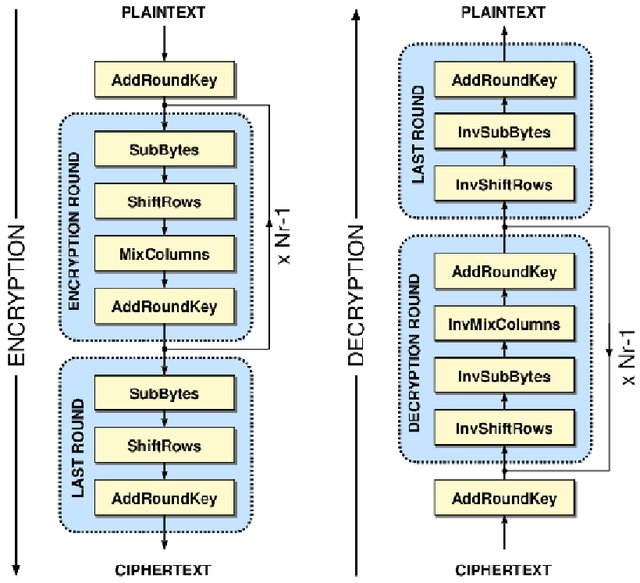
\includegraphics[width=0.85\textwidth]{img/AES.jpg}
	\caption{Схемы алгоритма AES}
	\label{fig:algo}
\end{figure}
\clearpage
